\documentclass[11pt,a4paper]{article}
\usepackage{fontspec}
\setmainfont{Times New Roman}
\setmonofont{Consolas}
\usepackage[margin=2.3cm]{geometry}
\usepackage{amsmath,amssymb,graphicx,booktabs,tabularx,array}
\usepackage{enumitem,caption,xurl}
\usepackage[unicode,hidelinks]{hyperref}
\setlength{\emergencystretch}{2em}
\setlength{\parskip}{3pt}
\setlist{itemsep=2pt,topsep=3pt,leftmargin=*}
\renewcommand{\figurename}{Hình}
\renewcommand{\tablename}{Bảng}
\renewcommand{\refname}{Tài liệu tham khảo}
\renewcommand{\abstractname}{Tóm tắt}
\newcommand{\code}[1]{\texttt{\detokenize{#1}}}
\newcolumntype{Y}{>{\raggedright\arraybackslash}X}
\title{\textbf{Dự báo chất lượng liên kết bằng mạng nơ-ron đồ thị cho định tuyến và bố trí UAV}}
\author{Nguyễn Đình Tâm\thanks{Tác giả liên hệ: \href{mailto:23521389@gm.uit.edu.vn}{23521389@gm.uit.edu.vn}.} \and Võ Công Vinh}
\date{Trường Đại học Công nghệ Thông tin, ĐHQG-HCM\\Tháng 11 năm 2026}
\begin{document}
\maketitle
\begin{abstract}
Nghiên cứu đánh giá giá trị của dự báo chất lượng liên kết đối với hai hành động trong mạng phương tiện bay không người lái (UAV): chọn tuyến dữ liệu và kích hoạt bố trí lại relay. Mạng nơ-ron đồ thị (GNN) dự báo tỷ lệ nhận probe trung bình trong năm giây tiếp theo từ vị trí, vận tốc và số đo liên kết nhân quả. Mô hình được học có giám sát từ dữ liệu lịch sử; mô hình đối chứng bỏ truyền thông điệp học được, nhưng vẫn giữ đặc trưng bậc nút và có ít tham số hơn. Hai nghiên cứu vòng kín được khóa trước khi chạy, mỗi nghiên cứu gồm 80 lượt validation và 192 lượt test mới trong ns-3.45, với chuỗi năm hoặc bảy UAV và các nhóm so sánh ghép cặp theo seed. Nghiên cứu định tuyến giữ relay đứng yên và cùng luật ghim tuyến, chỉ thay chất lượng hiện tại bằng dự báo. Trên 40 khối gradual test, dự báo đồ thị tăng tỷ lệ gói đến đích (PDR) 0,66 điểm phần trăm so với chất lượng hiện tại, khoảng tin cậy 95\% [0,38; 1,00], và tăng 0,38 điểm so với mô hình bỏ truyền thông điệp, khoảng tin cậy [0,12; 0,67]. Nghiên cứu điều khiển vị trí giữ cùng định tuyến và luật bố trí, chỉ thay điều kiện kích hoạt chuyển động. Dự báo giảm trung bình 0,20 giây chia cắt đồ thị probe so với kích hoạt phản ứng, khoảng tin cậy [$-1,05$; $1,45$], nên endpoint chính không đạt. Các nhóm di chuyển có khoảng 31 giây chia cắt so với 123 giây khi đứng yên, nhưng cần khoảng 637 m tổng quãng đường relay; đây là so sánh mô tả, không chứng minh lợi ích riêng của dự báo. Kết quả cho thấy cần đánh giá bộ dự báo cùng hành động cụ thể: GNN cải thiện định tuyến trong phạm vi đã thử, còn trigger vị trí chưa thể hiện lợi ích thêm rõ. Các giới hạn gồm telemetry tập trung chưa tranh chấp kênh, một seed huấn luyện, thay đổi phân phối chuyển động ở nghiên cứu vị trí và chưa có thử nghiệm bay thật.
\end{abstract}
\noindent\textbf{Từ khóa:} mạng UAV; mạng nơ-ron đồ thị; chất lượng liên kết; định tuyến; điều khiển vị trí.
\section{Giới thiệu}
Trong chuỗi UAV làm relay, suy giảm liên kết có thể gây mất gói hoặc chia cắt
nguồn--đích. Dự báo liên kết có thể hỗ trợ hai quyết định khác nhau: chọn đường
đi của gói tin và đặt lại vị trí relay. Một mô hình dự báo tốt hơn chưa tự động
chứng minh một bộ điều khiển tốt hơn; cần so sánh vòng kín với cùng luật hành
động và các kịch bản ghép cặp.

ETX đưa xác suất truyền thành công vào chi phí đường đi, thay cho chỉ đếm
hop~\cite{decouto}. Predictive-OLSR đã dùng vận tốc tương đối và GPS để điều
chỉnh chất lượng đường~\cite{rosati2013}. Vì vậy, đóng góp cần kiểm tra ở đây
là giá trị thêm của dự báo học được trong một hệ thống có kiểm soát, không
phải tuyên bố lần đầu dùng dự báo hoặc vị trí trong định tuyến UAV.
GraphSAGE cung cấp cơ chế học tổng hợp thông tin hàng xóm trên
đồ thị~\cite{graphsage}; nghiên cứu dùng một biến thể có đặc trưng cạnh
để hồi quy chất lượng liên kết.

OLSR-LCN kết hợp tuổi thọ liên kết, nhiễu và tải nút trong mở rộng
OLSR~\cite{liu2025}. Tối ưu quỹ đạo relay và công suất cũng đã được nghiên
cứu trong hệ thống mobile relaying~\cite{zeng2016}. Nghiên cứu hiện tại dùng
luật bố trí đơn giản để kiểm tra riêng thời điểm kích hoạt bằng dự báo;
không giải bài toán quỹ đạo tối ưu hoặc so sánh hiệu năng trực tiếp với các
công trình trên. Điểm nhấn là tách các phép so sánh, giữ seed và nguồn đã
khóa, kiểm tra lệnh thực thi, và phân biệt chất lượng dự báo với dịch vụ mạng.

Bài báo đặt hai câu hỏi. Thứ nhất, dự báo GNN có cải thiện tỷ lệ gói đến đích
(PDR) so với chất lượng hiện tại khi giữ nguyên luật chọn tuyến? Thứ hai,
dự báo có giảm số giây chia cắt khi giữ cùng định tuyến và cùng luật bố trí
relay, chỉ thay cơ chế kích hoạt chuyển động? Hai nghiên cứu kế tiếp được
ký hiệu v8 và v9 để liên kết với các hồ sơ thực nghiệm trong kho mã.
\section{Vật liệu và phương pháp}
Hình~\ref{fig:design} tóm tắt hai phép so sánh.
\begin{figure}[htbp]
\centering
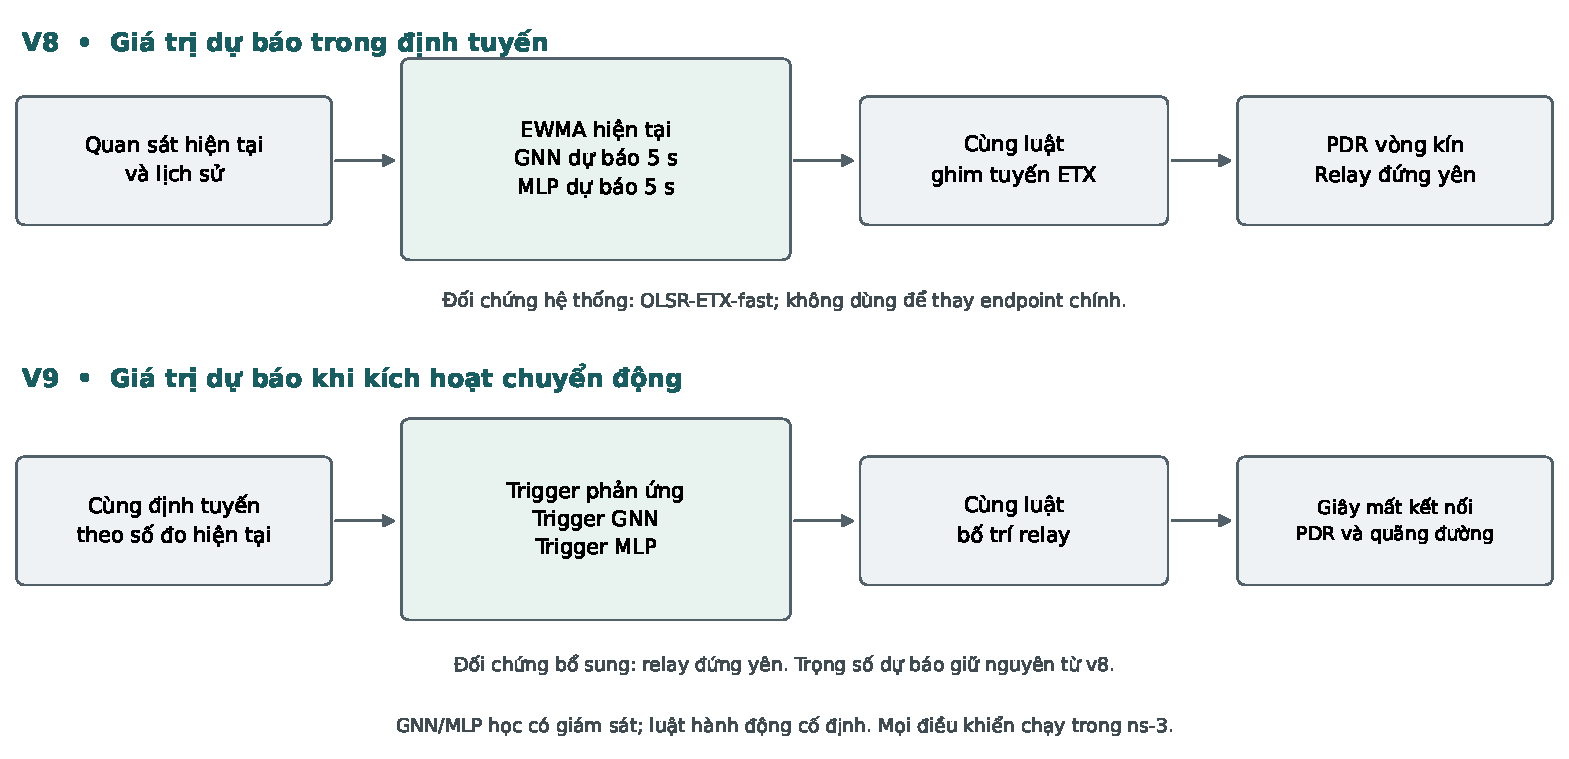
\includegraphics[width=\linewidth]{images/fig_v8_v9_design.pdf}
\caption{Thiết kế tách riêng dự báo cho định tuyến và dự báo cho kích hoạt chuyển động.}\label{fig:design}
\end{figure}
\subsection{Phát biểu bài toán}
Mạng ở thời điểm $t$ là đồ thị $G_t=(V,E_t)$ với $V$ là tập UAV. Mỗi cạnh
$e=(a,b)$ có chất lượng đo được $d_e(t)\in[0,1]$, là tỷ lệ nhận probe trong
cửa sổ một giây. Bộ ước lượng chất lượng tạo ra một đại lượng $x_e(t)$ dùng cho
quyết định, theo một trong hai họ:
\begin{align}
\text{đo và làm mượt:}\quad & x_e(t)=\alpha\, d_e(t)+(1-\alpha)\,x_e(t-1),\label{eq:ewma}\\
\text{dự báo học được:}\quad & x_e(t)=\hat g_e(t)\approx
\frac{1}{H}\sum_{\tau=t+1}^{t+H} d_e(\tau),\qquad H=5\ \text{giây}.\label{eq:fore}
\end{align}
Công thức~\eqref{eq:ewma} là EWMA một tham số; $\alpha=0{,}5$ là cấu hình của
các nghiên cứu trước và được dùng làm baseline của v8. Công thức~\eqref{eq:fore}
là bộ hồi quy GNN, học có giám sát từ dữ liệu lịch sử và chỉ dùng quan sát
nhân quả tới thời điểm $t$.

Hai hành động dùng chung $x$. Hành động định tuyến chọn đường
\begin{equation}
\pi_t=\arg\min_{P\in\mathcal{P}(s,d)}\ \sum_{e\in P}\frac{1}{\max(x_e(t),\varepsilon)},
\label{eq:etx}
\end{equation}
tức chi phí kiểu ETX~\cite{decouto} tính trên $x$ thay vì trên số đo thô, với
luật ghim tuyến có margin và dwell mô tả ở Mục~\ref{sub:v8}. Hành động bố trí
dùng chất lượng đường tốt nhất
\begin{equation}
Q(t)=\max_{P\in\mathcal{P}(s,d)}\ \min_{e\in P} x_e(t),
\label{eq:bottleneck}
\end{equation}
và kích hoạt một luật di chuyển relay cố định khi $Q(t)$ xuống dưới ngưỡng.

Phân biệt trung tâm của bài là giữa hai thước đo trên cùng một $x$. Chất lượng
\emph{dự báo} đo bằng sai số bình phương trung bình
$\mathrm{MSE}=\mathbb{E}\big[(x_e(t)-\frac{1}{H}\sum_\tau d_e(\tau))^2\big]$,
tính ngoại tuyến trên trace. Chất lượng \emph{dịch vụ} đo bằng PDR và số giây
chia cắt, tính trong vòng kín khi $x$ thật sự điều khiển~\eqref{eq:etx}
hoặc~\eqref{eq:bottleneck}. Câu hỏi của bài là hai thước đo này có xếp hạng các
bộ ước lượng theo cùng một thứ tự hay không.

\subsection{Môi trường và thiết kế thí nghiệm}
Thực nghiệm dùng ns-3.45~\cite{ns3}, Wi-Fi 802.11g và OLSR~\cite{rfc3626} trên chuỗi 5 hoặc 7 UAV.
Nguồn và đích ở hai đầu chuỗi; các nút còn lại làm relay. Mỗi episode dài
240 giây, luồng chính UDP 256 kbps, hai luồng nền 128 kbps. Hai bối cảnh gồm
static và gradual: đầu mút đứng yên hoặc di chuyển tách xa từ giây 30.
Binary và runtime kế thừa nghiên cứu trước, gồm baseline OLSR-ETX do nhóm
cài đặt và thời hạn ARP DeadTimeout 1 giây. Mọi arm dùng cùng binary,
kênh, lưu lượng và seed của khối tương ứng.
Vùng mô phỏng $1800\times1200$ m, độ cao 50--150 m. Khoảng cách ban đầu
giữa các nút liên tiếp danh định 24 m với jitter tối đa 0,72 m mỗi tọa độ.
Kênh dùng log-distance (số mũ 2,2, suy hao tham chiếu 40 dB tại 1 m) và
Nakagami ($m=3;1{,}5;1$ theo các dải khoảng cách dưới 96 m, 96--180 m,
trên 180 m). Công suất phát 20 dBm, tốc độ PHY cố định 6 Mbps. Tầm phủ
danh định 240 m dùng để đặt độ nhạy thu, không phải ngưỡng cắt liên kết
theo khoảng cách. Warmup 10 giây; probe broadcast cách 0,05 giây, tổng hợp
cửa sổ một giây; luồng chính gói 512 B, 15.000 gói mỗi episode.

Protocol được viết trước các mô phỏng mới. Mỗi pha đóng gói mã nguồn, mô
hình, seed plan và định danh runtime bằng SHA-256; test kế thừa đúng nguồn
và mô hình validation. Mỗi cell chạy một lần; queue bốn worker giữ lock
toàn server. Validation có 80 cell (hai static và tám gradual mỗi cấu hình,
bốn arm); test có 192 cell (bốn static và 20 gradual mỗi cấu hình, bốn arm).
Không chọn lại mô hình theo kết quả dịch vụ của validation hoặc test.

\subsection{Dự báo liên kết và đối chứng}
Mô hình dự báo tỷ lệ nhận probe trung bình trong năm giây tiếp theo, không
phải xác suất sống sót của liên kết. Dữ liệu phát triển gồm 48 trace HOLD
test v7 để fit và 20 trace HOLD validation v7 để chọn epoch. Các dữ liệu đã
quan sát này được coi hoàn toàn là dữ liệu phát triển cho nghiên cứu mới;
v8/v9 dùng seed độc lập đã kiểm toán. Mỗi episode có 236 gốc dự báo hợp lệ,
tạo 11.328 mẫu fit và 4.720 mẫu chọn epoch; các frame tương quan không được
coi là các lần lặp độc lập khi kiểm định hiệu quả điều khiển.

Đầu vào chỉ gồm quan sát hiện tại và quá khứ. Tám đặc trưng nút gồm tọa độ
tương đối với tâm đội hình, vận tốc, bậc hàng xóm và tỷ lệ nhận trung bình.
Bảy đặc trưng cạnh gồm khoảng cách, RSSI, tỷ lệ nhận hiện tại, EWMA hệ số
0,5, chênh tỷ lệ nhận, vận tốc tách xa và độ lớn vận tốc tương đối. Tọa độ
và khoảng cách chia 240 m; vận tốc chia 10 m/s; RSSI biến đổi thành
$(RSSI+90)/40$, giá trị thiếu mã hóa $-100$ dBm. Cạnh truyền thông điệp có
tỷ lệ nhận hiện tại ít nhất 0,1. Không đọc quỹ đạo nhiệm vụ trong tương lai.

Edge-SAGE gồm hai lớp tổng hợp trung bình với đặc trưng cạnh, 64 chiều và
ReLU; bộ giải mã cặp nút 64 chiều và sigmoid, đối xứng hóa logits. GNN có
19.137 tham số. MLP bỏ hai nhánh truyền thông điệp học được, còn 13.505 tham
số; vẫn giữ đặc trưng bậc nút. Vì thế ablation chưa tách riêng tác động của
truyền thông điệp khỏi khác biệt dung lượng mô hình. Cả hai dùng MSE, Adam
lr 0,001, weight decay $10^{-5}$, batch 128, clip norm 5, tối đa 60 epoch,
patience 10, seed 20261123. GNN/MLP chọn epoch 58/59. Sai số lớn nhất giữa
suy luận NumPy và PyTorch trên 40 snapshot kiểm tra là $1{,}19\times10^{-7}$.
Đây là học có giám sát; các nghiên cứu không dùng học tăng cường.

\subsection{Nghiên cứu định tuyến v8}\label{sub:v8}
Bốn arm là chất lượng hiện tại (\code{lq-route}), dự báo GNN
(\code{gnn-route}), dự báo MLP (\code{mlp-route}) và OLSR-ETX-fast.
Ba arm ghim tuyến giữ cùng luật ETX với margin 1,0, warmup ba bước và dwell
năm giây; kiểm tra liên kết hỏng vẫn dựa trên tỷ lệ nhận hiện tại dưới 0,1.
ETX-fast dùng HELLO 0,5 s, TC 1,25 s đã chọn ở v7. Relay đứng yên; tốc độ
mỗi đầu mút gradual có giá trị danh định 1 m/s, nhân hệ số [0,85; 1,15] theo
layout seed. Nguồn đi theo chiều $+y$, đích theo chiều $-y$; cùng seed giữ
cùng chuyển động đầu mút giữa các arm. Validation chỉ kiểm tra kỹ thuật: đủ cell,
đúng tuyến, cờ simulator, forecast, bộ đếm và luồng nền, không blackout khởi
động và không di chuyển relay. Go không phụ thuộc chênh PDR.

Ba bước kiểm định theo thứ tự cố định là PDR GNN trừ hiện tại, GNN trừ MLP,
rồi GNN trừ ETX-fast. Một bước đạt khi cận dưới CI 95\% dương; chỉ diễn giải
khẳng định khi mọi bước trước đạt. MSE test được đo riêng cho GNN, MLP và
EWMA trên cùng các trace \code{lq-route}, tách khỏi PDR vòng kín.

\subsection{Nghiên cứu vị trí v9}
V9 giữ nguyên trọng số v8 và giữ định tuyến theo chất lượng hiện tại ở mọi
arm. Các arm là relay đứng yên, kích hoạt di chuyển phản ứng, kích hoạt bằng
GNN và kích hoạt bằng MLP. Chất lượng đường tốt nhất là $Q=\max_P\min_{e\in P}q_e$.
Sau ba frame, reactive kích hoạt nếu EWMA hiện tại có $Q<0{,}70$ trong hai
frame liên tiếp; GNN/MLP dùng thêm điều kiện tương tự trên dự báo. Cạnh dự
báo chỉ được dùng nếu số đo hiện tại ít nhất 0,1.

Các relay được xếp theo hình chiếu lên đường nối đầu mút hiện tại rồi hướng
tới các điểm chia đều đoạn đó. Giới hạn: 8 m/s, 400 m mỗi relay, deadband
1 m, tối đa mười bước mỗi đợt và nghỉ năm bước. Dừng sớm sau ba frame có
chất lượng hiện tại và dự báo (nếu có) ít nhất 0,80. Kiểm tra khoảng cách
nhỏ nhất trong bước phải đạt 5 m; nếu không, lệnh chuyển động relay bằng 0.
Luật này giống nhau ở mọi arm có chuyển động, chỉ khác trigger.

Tốc độ danh định mỗi đầu mút gradual tăng lên 2 m/s, vẫn giữ hệ số ngẫu nhiên
theo seed như v8, để tạo thách thức chia cắt; khác phân phối fit 1 m/s.
Validation đòi kỹ thuật/an toàn đạt và ít nhất 8/16
baseline gradual đứng yên mất kết nối ít nhất năm giây. Nếu không đạt thì
dừng test, không chỉnh lại tốc độ trong cùng nghiên cứu.

Endpoint chính là số giây mất kết nối của reactive trừ GNN; sau đó xét PDR
GNN trừ reactive, rồi số giây mất kết nối của MLP trừ GNN. Mất kết nối là
nguồn và đích khác thành phần liên thông trong đồ thị probe ngưỡng 0,5, đếm
trên frame 1--240. Số giây OLSR không có tuyến và PDR là các đại lượng khác.
Đây là chia cắt theo ngưỡng đồ thị đo được, không phải chứng minh hoàn toàn
không có gói vô tuyến nào có thể truyền giữa các thành phần.
Quãng đường, outage dài nhất, số đợt di chuyển và PDR luồng nền là mô tả.

\subsection{Phân tích thống kê và chi phí}
Mỗi so sánh giữ bốn arm cùng khối seed; bootstrap 10.000 lần trên 40 khối
gradual test, 20 mỗi cấu hình, cân bằng n5/n7, RNG 20261120. Bootstrap~\cite{efron1993}
được áp dụng ở cấp kịch bản để giữ tương quan giữa các arm. Kết quả âm và
các bước bị đóng cổng vẫn được trình bày. CI chứa 0 không chứng minh tương
đương. Kết quả static chỉ mô tả với tám khối.

Collector đo thời gian toàn bộ quyết định trên máy ảo KVM tám vCPU (model
Intel Xeon Silver 4110 2,10 GHz), chạy bốn worker, mỗi worker giới hạn thư
viện tính toán về một luồng. Probe phát trong mọi arm; telemetry và lệnh tập trung chưa được
truyền thành gói cạnh tranh kênh. Không quy thời gian tính thành độ trễ điều
khiển đầu cuối, số byte thành airtime, hoặc quãng đường thành năng lượng.

Chi phí báo hiệu được đo ở nghiên cứu v7 với cùng binary và runtime, nên các
con số sau áp dụng cho cấu hình của v8: OLSR thuần khoảng 0,29 kB/s, OLSR-ETX
0,44 kB/s, OLSR-ETX với HELLO 0,5 giây 1,78 kB/s, và ghim tuyến khoảng
5,55 kB/s gồm OLSR dự phòng 0,29 kB/s, probe 5,02 kB/s và báo cáo về bộ điều
khiển ước lượng 0,25 kB/s. Đây là byte tầng IP cộng phần báo cáo ước lượng,
không quy đổi thành phần trăm dung lượng kênh. Probe được phát ở mọi arm nên
airtime của probe là chung giữa các arm, nhưng chỉ được hạch toán vào chi phí
của các phương pháp sử dụng probe. Phần báo cáo tập trung chưa chiếm kênh trong
mô phỏng. Vì vậy mọi so sánh giữa ghim tuyến và OLSR-ETX trong bài phải được
đọc như giới hạn trên của một bộ điều khiển tập trung lý tưởng hóa một phần.

\section{Kết quả}
\subsection{Dự báo cho định tuyến}

Validation v8 có 80/80 cell hợp lệ; đạt go và test có 192/192 cell hợp lệ.

Bảng~\ref{tab:v8primary} trình bày các phép so sánh theo thứ tự đã khóa.

\begin{table}[htbp]
\centering\small
\begin{tabularx}{\linewidth}{@{}Yp{1.8cm}p{3.4cm}p{1.7cm}@{}}
\toprule
\textbf{So sánh}&\textbf{Chênh lệch}&\textbf{CI 95\%}&\textbf{Cổng}\\\midrule
H1: \code{gnn-route} $-$ \code{lq-route}&0,66&[0,38; 1,00]&Đạt\\
H2: \code{gnn-route} $-$ \code{mlp-route}&0,38&[0,12; 0,67]&Đạt\\
H3: \code{gnn-route} $-$ \code{olsr-etx-fast}&5,75&[5,07; 6,45]&Đạt\\
\bottomrule
\end{tabularx}
\caption{Test định tuyến: PDR tính bằng điểm phần trăm. Mỗi so sánh dùng 40 khối gradual mới.}\label{tab:v8primary}
\end{table}


Endpoint chính đạt; các bước sau tuân theo cổng thứ tự trong bảng. Toàn vẹn tuyến đúng 144/144 episode được kiểm tra; các kiểm tra kỹ thuật đều đạt.

Bảng~\ref{tab:v8meanspaper} ghi PDR, thời gian mất kết nối và quãng đường của từng arm.

\begin{table}[htbp]
\centering\small
\begin{tabularx}{\linewidth}{@{}Yp{3.4cm}p{2.2cm}p{2.5cm}@{}}
\toprule
\textbf{Arm}&\textbf{PDR (\%, TB $\pm$ SD)}&\textbf{Mất kết nối (s)}&\textbf{Quãng đường (m)}\\\midrule
\code{gnn-route}&96,01 $\pm$ 2,58&31,65&0,00\\
\code{lq-route}&95,35 $\pm$ 2,92&31,77&0,00\\
\code{mlp-route}&95,64 $\pm$ 2,68&31,77&0,00\\
\code{olsr-etx-fast}&90,26 $\pm$ 4,38&35,90&0,00\\
\bottomrule
\end{tabularx}
\caption{Mô tả gradual test v8; PDR trung bình và SD theo episode, các cột còn lại là trung bình. Quãng đường cộng trên relay, không đại diện năng lượng.}\label{tab:v8meanspaper}
\end{table}


Trên cùng trace test \code{lq-route}, MSE GNN, MLP và EWMA lần lượt là 0,0007846; 0,0011143; 0,0012738. Số lệnh đổi tuyến trên toàn test của GNN, MLP và EWMA là 95; 208; 359. GNN trừ EWMA có chênh thời gian mất kết nối $-0{,}13$ giây, CI 95\% [$-0{,}97$; $0{,}68$]; không cho thấy giảm chia cắt rõ. Static có PDR gần 100\% và chênh GNN trừ EWMA bằng 0 trên tám khối. Chênh PDR luồng nền GNN trừ EWMA là 0,005 điểm phần trăm, CI 95\% [$-0{,}119$; $0{,}123$], chỉ mô tả.

Thời gian toàn bộ quyết định GNN trung vị 4,92 ms, phân vị 95\% 13,83 ms; EWMA trung vị 3,00 ms. Đây là số đo CPU server, chưa gồm telemetry và truyền lệnh.

\subsection{Dự báo cho kích hoạt chuyển động}

Validation v9 có 80/80 cell hợp lệ; đạt go và test có 192/192 cell hợp lệ.

Bảng~\ref{tab:v9primary} trình bày các phép so sánh theo thứ tự đã khóa.

\begin{table}[htbp]
\centering\small
\begin{tabularx}{\linewidth}{@{}Yp{1.8cm}p{3.4cm}p{1.7cm}@{}}
\toprule
\textbf{So sánh}&\textbf{Chênh lệch}&\textbf{CI 95\%}&\textbf{Cổng}\\\midrule
H1: \code{reactive-motion} $-$ \code{gnn-motion}&0,20&[-1,05; 1,45]&Không đạt\\
H2: \code{gnn-motion} $-$ \code{reactive-motion}&0,34&[-0,32; 1,04]&Mô tả\\
H3: \code{mlp-motion} $-$ \code{gnn-motion}&1,23&[0,10; 2,52]&Mô tả\\
\bottomrule
\end{tabularx}
\caption{Test vị trí: H1/H3 là giây mất kết nối tiết kiệm được, H2 là chênh PDR theo điểm phần trăm. Mỗi so sánh dùng 40 khối gradual mới.}\label{tab:v9primary}
\end{table}


Endpoint chính không đạt; các bước sau tuân theo cổng thứ tự trong bảng. Toàn vẹn tuyến đúng 192/192 episode được kiểm tra; các kiểm tra kỹ thuật đều đạt.

Bảng~\ref{tab:v9meanspaper} ghi PDR, thời gian mất kết nối và quãng đường của từng arm.

\begin{table}[htbp]
\centering\small
\begin{tabularx}{\linewidth}{@{}Yp{3.4cm}p{2.2cm}p{2.5cm}@{}}
\toprule
\textbf{Arm}&\textbf{PDR (\%, TB $\pm$ SD)}&\textbf{Mất kết nối (s)}&\textbf{Quãng đường (m)}\\\midrule
\code{gnn-motion}&88,60 $\pm$ 4,27&31,25&636,76\\
\code{mlp-motion}&88,08 $\pm$ 4,93&32,48&638,97\\
\code{reactive-motion}&88,26 $\pm$ 4,39&31,45&637,48\\
\code{route-only}&59,89 $\pm$ 4,91&123,42&0,00\\
\bottomrule
\end{tabularx}
\caption{Mô tả gradual test v9; PDR trung bình và SD theo episode, các cột còn lại là trung bình. Quãng đường cộng trên relay, không đại diện năng lượng.}\label{tab:v9meanspaper}
\end{table}


\begin{figure}[htbp]\centering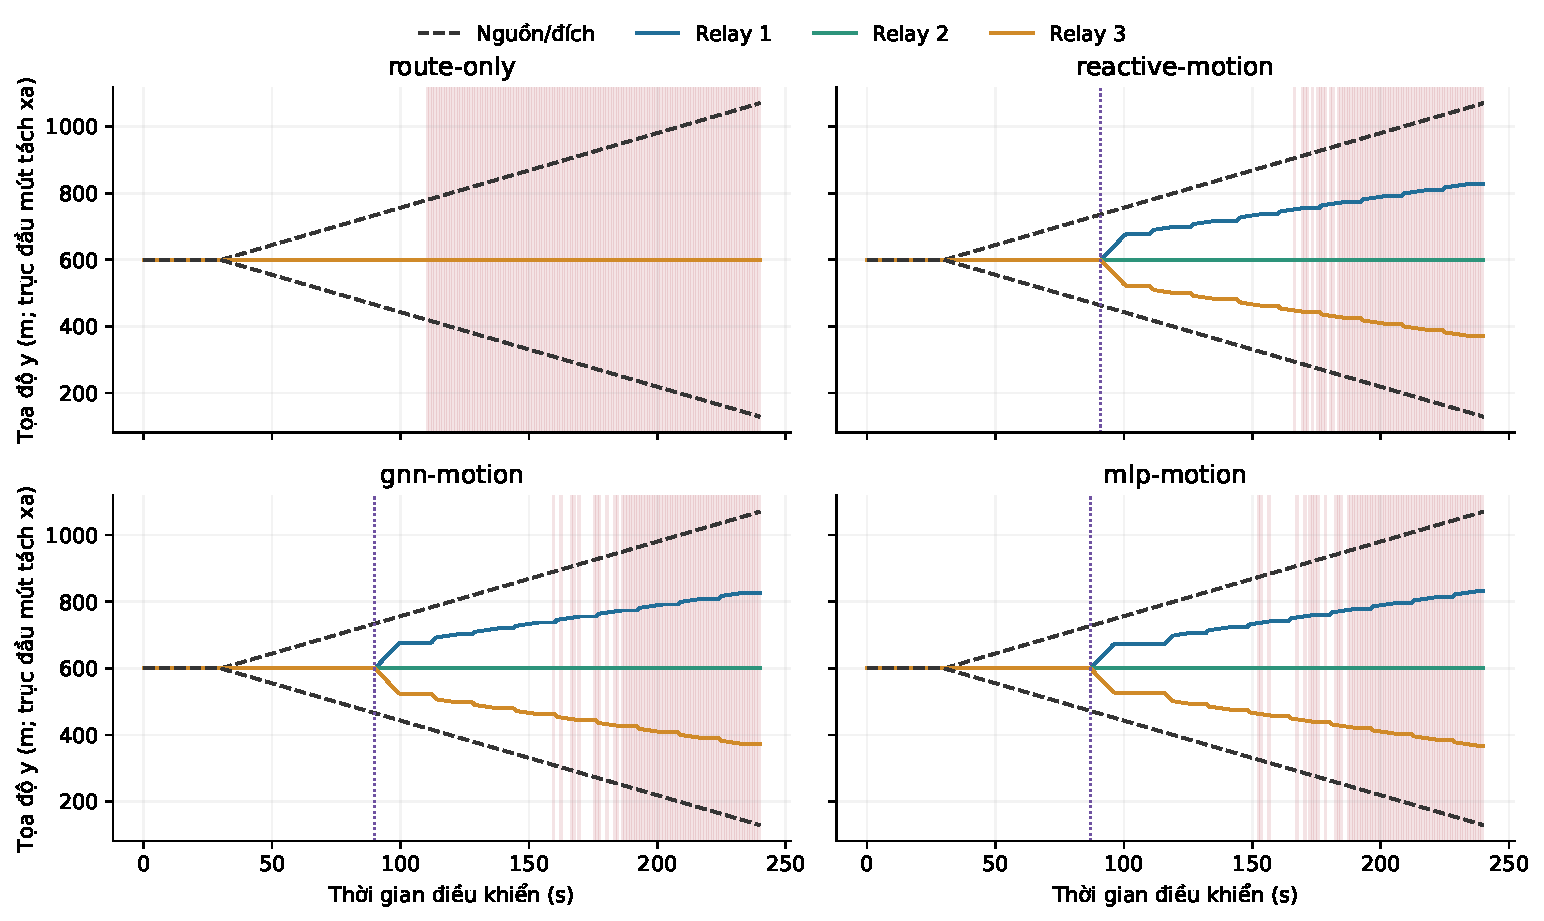
\includegraphics[width=\linewidth]{images/fig_v9_motion_example.pdf}\caption{Ví dụ n5 gradual có layout seed nhỏ nhất, lấy đủ bốn arm; vùng đỏ nhạt là mất kết nối theo probe, đường tím là lần chuyển động đầu tiên. Không chọn seed theo kết quả thuận lợi.}\label{fig:motionexample}\end{figure}

Hình~\ref{fig:motionexample} minh họa hành động thực thi; kết luận lấy từ toàn bộ các khối kịch bản. Số episode có chuyển động trong gradual: \code{gnn-motion}: 40/40; \code{mlp-motion}: 40/40; \code{reactive-motion}: 40/40; \code{route-only}: 0/40.

\section{Thảo luận}
Hai nghiên cứu cho các kết luận khác nhau về cùng một bộ dự báo. Với luật
ghim tuyến, GNN đem lại lợi ích thêm nhỏ nhưng CI dương; so sánh với MLP
ủng hộ lợi ích của cấu hình GNN đã thử, chưa cô lập riêng ảnh hưởng của
truyền thông điệp vì số tham số khác nhau. Việc ít đổi tuyến hơn là một
giải thích khả dĩ, chưa được can thiệp kiểm tra riêng.

Với điều khiển vị trí, endpoint chính không đạt. Kết quả GNN--MLP có CI
riêng lẻ dương chỉ mang tính mô tả vì cổng đầu tiên đã đóng. Trigger reactive
dùng ngưỡng chất lượng 0,70, thường đã hành động trước chia cắt đồ thị
ngưỡng 0,5; nó không chờ đến khi mất liên lạc mới di chuyển. Do đó dư địa
cho dự báo năm giây có thể nhỏ. Chuyển miền vận tốc và việc mô hình chỉ
được fit trên relay đứng yên cũng là các khả năng cần kiểm tra tiếp.
Không có phép thử riêng để chọn một giải thích làm nguyên nhân duy nhất.

Di chuyển giảm mạnh mất kết nối so với relay đứng yên ở kịch bản nhanh,
nhưng lợi ích đó chưa chứng minh phần đóng góp riêng của dự báo. Chi phí
hình học tương tự giữa trigger GNN và reactive, trong khi GNN cần tính
toán và telemetry bổ sung. CI chứa 0 không chứng minh tương đương; cũng
không đủ căn cứ để thêm một mô hình phức tạp chỉ từ chênh lệch điểm ước lượng.
Không thay ngưỡng hoặc huấn luyện lại sau khi thấy test. Hướng tiếp theo
là thu thập dữ liệu relay di chuyển, kiểm tra hiệu chuẩn và báo hiệu trên
kênh, rồi đăng ký một nghiên cứu mới nếu học chính sách bằng RL.


Các giới hạn đã xác định gồm một họ topology chuỗi relay, bộ điều khiển
tập trung chưa chịu mất thông điệp, lưu lượng telemetry chưa tranh chấp kênh,
và chưa có thử nghiệm UAV thật. Ở nghiên cứu vị trí, tốc độ đầu mút khác dữ
liệu huấn luyện, đồng thời relay chuyển từ đứng yên trong dữ liệu fit sang
di chuyển. Mô hình không được huấn luyện để so sánh các hành động phản thực;
nó chỉ kích hoạt một luật bố trí cố định. Quãng đường di chuyển chỉ là chi phí hình học, chưa được
chuyển đổi thành năng lượng.
Mỗi mô hình chỉ có một seed huấn luyện; CI bootstrap theo kịch bản điều kiện
trên trọng số đã khóa, chưa mô tả biến thiên giữa các lần huấn luyện.
\section{Kết luận}
Trong hai nghiên cứu đã khóa trên chuỗi 5/7 UAV, GNN hồi quy năm giây
cải thiện PDR khi dùng cho lựa chọn tuyến, nhưng chưa thể hiện lợi ích
thêm rõ khi chỉ kích hoạt một luật bố trí relay chung. Kết luận về dự báo
cần gắn với hành động và baseline cụ thể; độ chính xác dự báo cao hơn
không thay thế thí nghiệm dịch vụ vòng kín. Hệ thống và bằng chứng hiện
có phù hợp cho đánh giá mô phỏng trong phạm vi công bố, chưa xác nhận
khả năng triển khai bay thật.
\section*{Thông tin tác giả và dữ liệu}
Nhóm cảm ơn ThS. Đặng Lê Bảo Chương đã hướng dẫn đề tài.
Nguyễn Đình Tâm là người thực hiện chính và tác giả liên hệ.
Kho mã nền: \url{https://github.com/kaing615/UAV-link-quality-routing-support}.
Gói tái lập đi kèm bản thảo chứa nguồn đóng gói, mô hình, kế hoạch seed,
kết quả và manifest SHA-256; trace đầy đủ được lưu trên server của nhóm.
\begin{thebibliography}{9}
\bibitem{decouto} D. S. J. De Couto, D. Aguayo, J. Bicket, R. Morris.
A high-throughput path metric for multi-hop wireless routing.
\textit{Proc. ACM MobiCom}, 2003.
\bibitem{rosati2013} S. Rosati, K. Kruzelecki, L. Traynard, B. Rimoldi.
\textit{Speed-Aware Routing for UAV Ad-Hoc Networks}.
arXiv:1307.6350, 2013. \url{https://arxiv.org/abs/1307.6350}.
\bibitem{graphsage} W. L. Hamilton, R. Ying, J. Leskovec.
Inductive representation learning on large graphs.
\textit{NeurIPS}, 2017. \url{https://arxiv.org/abs/1706.02216}.
\bibitem{liu2025} J. Liu, P. Gong, H. Yang, S. Li, X. Gao.
Cross-Layer Optimized OLSR Protocol for FANETs in Interference-Intensive Environments.
\textit{Drones}, 9(11):778, 2025. \url{https://doi.org/10.3390/drones9110778}.
\bibitem{zeng2016} Y. Zeng, R. Zhang, T. J. Lim.
Throughput maximization for UAV-enabled mobile relaying systems.
\textit{IEEE Transactions on Communications}, 64(12):4983--4996, 2016.
\bibitem{rfc3626} T. Clausen, P. Jacquet.
\textit{Optimized Link State Routing Protocol (OLSR)}. RFC 3626, 2003.
\url{https://www.rfc-editor.org/rfc/rfc3626}.
\bibitem{efron1993} B. Efron, R. J. Tibshirani.
\textit{An Introduction to the Bootstrap}. Chapman \& Hall, 1993.
\end{thebibliography}
\end{document}
